\newpage
\chapter{Interfacing a model with the PSMILe library}
\label{sec_modelinterfacing}

At run-time, the OASIS3 coupling layer supports coupling data
between two components as well as interpolation and transformation
of coupled fields. To communicate with OASIS3 or directly between the component
models, different communication techniques have been historically
developed. The technique used for one particular run is defined by the
user with the keyword \$CHANNEL in the configuration file {\it namcouple} 
(see chapter
\ref{sec_namcouple}). In OASIS3, direct coupling is supported 
based on MPI1 or MPI2 (not yet supported) message passing implementation
using the associated model interface library PSMILe.  For
a practical toy model using the PSMILe library, see the sources in
{\tt /oasis3/examples/toyoasis3/src} and more details in
chapter \ref{sec_compilationrunning}.


%\vspace*{0.5cm}

 To communicate with OASIS3 or directly with another component model
  or to perform I/O actions, a component model needs to be interfaced
  with the PRISM System Model Interface library, PSMILe, which sources
  can be found in {\tt oasis3/lib/psmile} directory. PSMILe supports:

\begin{itemize}
\item parallel communication between parallel component models
\item automatic sending and receiving actions at appropriate times
 following user's choice indicated in the {\it namcouple},
\item time integration or accumulation of the coupling fields,
\item limited transformations such as mapping (interpolation) between grids
\item I/O actions from/to files.
\end{itemize}

 To adapt a component model to PSMILe, specific calls of
 the following classes have to be implemented in the code:

\begin{enumerate}
\item Initialisation (section \ref{subsubsec_Initialisation})
\item Grid data file definition (section \ref{subsubsec_griddef})
\item Partition definition (section \ref{subsubsec_Partition})
\item I/O-coupling field declaration (section \ref{subsubsec_Declaration})
\item End of definition phase (section \ref{subsubsec_Endofdefinition})
\item I/O-coupling field sending and receiving (section
\ref{subsubsec_sendingreceiving})
\item Termination (section \ref{subsubsec_Termination})
\end{enumerate}

Finally, in section \ref{subsubsec_Algoritms}, different coupling
algorithms are illustrated, and explanations are given on how to
reproduce them with PSMILe by defining the appropriate indices of
lag and sequence for each coupling field.

\section{Use}
\label{subsubsec_Use}
%{Use}

To use prism, a user needs to add 

\begin{itemize}

\item {\tt USE mod\_prism}

 ** OR **

\item {\tt USE mod\_oasis}
 
\end{itemize}

Both use statements are valid and use of just one or the other
is recommended in a particular model.  Different models in a single 
coupled configuration can use either prism or oasis interfaces.  
A single use statement now provides all the methods
that previously required multiple use statements.  The interface,
methods, datatypes, and capabilities are identical for either the
mod\_prism or mod\_oasis interfaces.  The only difference is the name
of the interface.  mod\_prism is provided
for backwards compatability with prior versions of oasis.  mod\_oasis
provides a set of updated interface names that will continue to evolve
in the future.  In the following sections, both the mod\_prism
and mod\_oasis name will be identified but descriptions will be based
on the mod\_prism interface.  the mod\_oasis interface names can be user 
interchangably in those descriptions.

\section{Initialisation}
\label{subsubsec_Initialisation}
%{Initialisation}

All processes of the component model initialise the coupling and, if
required, retrieve a local communicator for the component model
internal parallelisation.

\begin{itemize}

\item {\tt CALL prism\_init\_comp\_proto (compid, model\_name, ierror)} 
\item {\tt CALL oasis\_init\_comp        (compid, model\_name, ierror)} 

 \begin{itemize}
   \item {\tt compid [INTEGER; OUT]}: component model ID 
   \item {\tt model\_name [CHARACTER*6; IN]}: name of calling model (as in
  {\em namcouple}) 
   \item {\tt ierror [INTEGER; OUT]}: returned error code.
 \end{itemize}
 
Routine called by all component model processes, which initialises the
coupling.\footnote{The model may call MPI\_Init explicitly, but if so, has to
call it before calling {\tt prism\_init\_comp\_proto}; in this case, the
model also has to call MPI\_Finalize explicitly, but only after calling
{\tt prism\_terminate\_proto}.}

\item {\tt CALL prism\_get\_localcomm\_proto (local\_comm, ierror )}
\item {\tt CALL oasis\_get\_localcomm        (local\_comm, ierror )}

 \begin{itemize}
   \item {\tt local\_comm [INTEGER; OUT]}: value of local communicator
   \item {\tt ierror [INTEGER; OUT]}: returned error code.
  \end{itemize}

  If needed, routine called by all model processes  
  to get the value of a local communicator to be used by the
  model for its internal parallelisation (CLIM-MPI1 communication technique only). 

  With CLIM-MPI1, all component models started in a
  pseudo-MPMD mode share automatically the same MPI\_COMM\_WORLD
  communicator.  Another communicator has to be used for the internal
  parallelisation of each model. OASIS3 creates this model local
  communicator based on the name of the calling model; its value is returned
  as the first argument of prism\_get\_localcomm\_proto routine.

  With CLIM-MPI2, OASIS3 executable spawns the component model executables at the
  beginning of the run; 
  the components keep their internal parallelisation context unchanged 
  with respect to their standalone mode. In this case, calling the prism\_get\_localcomm\_proto 
  routine is useless but if called, the communicator MPI\_COMM\_WORLD will be returned as
  local communicator.

\end{itemize}

\section{Grid data file definition}
\label{subsubsec_griddef}

The grid data files {\em grids.nc, masks.nc} and {\em areas.nc} can be
created by the user before the run or can be written directly at run
time by the master process of each component model (except when
  OASIS3 is used in ``IPSL'' parallel mode, see section
  \ref{sec_ipslpara_mode}).

  If written by the component models, the writing of those grid files
  is driven by OASIS3 main process. It first checks whether the binary
  file {\em grids} or the netCDF file {\em grids.nc} exists (if it is
  the case, it assumes that {\em areas} or {\em areas.nc} and {\em
    masks} or {\em masks.nc} files exist too), or if writing is
  needed. If {\em grids} or {\em grids.nc} exists, it must contain all
  grid information from all models; the file will not be completed or
  overwritten even if the following routines are explicitely
  called. If {\em grids} or {\em grids.nc} does not exist, each model
  must write its grid, mask and area definition in the grid data files
  with the following routines.

The coupler sends the information on whether or not writing is needed
to the mo\-dels following an OASIS3 internal order (below
prism\_start\_grids\_writing called by the component master process). 
If the grid data files already exist in the working directory, nothing
happens when the component model calls the {\tt prism\_write\_grid}, 
{\tt prism\_write\_corner}, {\tt prism\_write\_ang}, 
{\tt prism\_write\_mask}, \newline{\tt prism\_write\_area} routines;
the grid information is NOT overwritten in the grid files. If
writing is needed, the first model creates the files, writes the data
arrays when calling the appropriate routines,
and then sends a termination flag to the coupler (below \break {\tt
prism\_terminate\_grids\_writing} call). The coupler will then send the
starting flag to the next model; this ensures that only one model
accesses the files at a time.

This section describes the PSMILe routines to be called by the
master process of each component model to write, at run time, the whole
grid information to the grid data files. These routines have to
be called just after {\tt prism\_init\_comp\_proto}.

As an example, see the TOYOASIS3 coupled model components that 
use these routines to write the grid data
files (effective if \texttt{gridswr=1} in the running script
\texttt{run\_toyoasis3},  
%XXXXX or \texttt{RUN\_toyclim\_$<$expid$>$} 
see section \ref{sec_coupled_mode}).

%To run a toy experiment
%into which the component models write those files, execute the
%script prism/util/running/toyclim/sc\_run\_toyclim\_grid. 

\begin{itemize}
  
\item {\tt CALL  prism\_start\_grids\_writing (flag)}
\item {\tt CALL  oasis\_start\_grids\_writing (flag)}
        
  \begin{itemize}
    \item {\tt flag [INTEGER; OUT]}:  returns 1 or 0 if grids writing is
    needed or not needed
  \end{itemize}
Initialisation of grids writing.

\item {\tt CALL prism\_write\_grid (cgrid, nx, ny, lon, lat)}
\item {\tt CALL oasis\_write\_grid (cgrid, nx, ny, lon, lat)}
        
 \begin{itemize}
    \item {\tt cgrid [CHARACTER*4; IN]}: grid name prefix (see
    \ref{subsec_namcouplesecond})
    \item {\tt nx [INTEGER; IN]} : first grid dimension (x)
    \item {\tt ny [INTEGER; IN]} : second grid dimension (y)
    \item {\tt lon [REAL, DIMENSION(nx,ny); IN)} : array of longitudes
      (degrees East) 
    \item {\tt lat [REAL, DIMENSION(nx,ny); IN)} : array of latitudes
    (degrees North)
 \end{itemize}

 Writing of the model grid longitudes and latitudes. Longitudes must
 be given in degrees East in the interval -360.0 to 720.0. Latitudes
 must be given in degrees North in the interval -90.0 to 90.0. Note
 that if some grid points overlap, it is recommended to define those
 points with the same number (e.g. 90.0 for both, not 450.0 for one
 and 90.0 for the other) to ensure automatic detection of overlap by OASIS
 (which is essential to have a correct conservative remapping
 \texttt{SCRIPR/CONSERV}, see section \ref{subsec_interp}). 


\item {\tt CALL prism\_write\_corner (cgrid, nx, ny, nc, clon, clat)}
\item {\tt CALL oasis\_write\_corner (cgrid, nx, ny, nc, clon, clat)}

 \begin{itemize}
    \item {\tt cgrid [CHARACTER*4; IN]}: grid name prefix
    \item {\tt nx [INTEGER; IN]} : first grid dimension (x)
    \item {\tt ny [INTEGER; IN]} : second grid dimension (y)
    \item {\tt nc [INTEGER; IN]} : number of corners per grid cell (always 4 in the version)
    \item {\tt lon [REAL, DIMENSION (nx,ny,nc);IN]} : array of corner
    longitudes (in degrees\_East)
    \item {\tt lat [REAL, DIMENSION (nx,ny,nc);IN]} : array of corner
    latitudes (in degrees\_North)
 \end{itemize}

 Writing of the grid cell corner longitudes and latitudes
 (counterclockwise sense). Longitudes must be given in degrees East in
 the interval -360.0 to 720.0. Latitudes must be given in degrees
 North in the interval -90.0 to 90.0. Note also that cells larger than
 180.0 degrees in longitude are not supported. Writing of corners is
 optional as corner information is needed only for some
 transformations (see section \ref{subsec_griddata}). If called,
 prism\_write\_corners needs to be called after prism\_write\_grids.

\item {\tt CALL prism\_write\_angle (cgrid, nx, ny, angle)}
\item {\tt CALL oasis\_write\_angle (cgrid, nx, ny, angle)}

 \begin{itemize}
    \item {\tt cgrid [CHARACTER*4; IN]}: grid name prefix
    \item {\tt nx [INTEGER; IN]} : first grid dimension (x)
    \item {\tt ny [INTEGER; IN]} : second grid dimension (y)
    \item {\tt angle [REAL, DIMENSION (nx,ny);IN]} : array of angles
 \end{itemize}

 Writing of the grid angles; needed only if coupling fields
 are vector fields defined on a grid which has a local coordinate system not oriented in 
 the zonal and meridional directions. The angle is defined as the angle between the vector
 first component and the zonal direction. See SCRIPR/CONSERV in section \ref{subsec_preproc}.

 If called,
 prism\_write\_angle needs to be called after prism\_write\_grids.

\item {\tt CALL prism\_write\_mask (cgrid, nx, ny, mask)}
\item {\tt CALL oasis\_write\_mask (cgrid, nx, ny, mask)}

 \begin{itemize}
    \item {\tt cgrid [CHARACTER*4; IN]}: grid name prefix 
    \item {\tt nx [INTEGER; IN]} : first grid dimension (x)
    \item {\tt ny [INTEGER; IN]} : second grid dimension (y)
    \item {\tt mask [INTEGER, DIMENSION(nx,ny) ;IN]} : mask array (0 - not masked, 1 - masked)
 \end{itemize}
Writing of the model grid mask.

\item {\tt CALL prism\_write\_area (cgrid, nx, ny, area)}
\item {\tt CALL oasis\_write\_area (cgrid, nx, ny, area)}

 \begin{itemize}
    \item {\tt cgrid [CHARACTER*4; IN]}: grid name prefix
    \item {\tt nx [INTEGER; IN]} : first grid dimension (x)
    \item {\tt ny [INTEGER; IN]} : second grid dimension (y)
    \item {\tt area [REAL, DIMENSION(nx,ny); IN]} : array of grid cell areas
 \end{itemize}
Writing of the model grid cell areas. Writing of areas is optional as
area information is needed only for some transformations (see section
\ref{subsec_griddata}).

\item {\tt CALL prism\_terminate\_grids\_writing()}
\item {\tt CALL oasis\_terminate\_grids\_writing()}

Termination of grids writing. A flag stating that all needed grid
information was written will be sent to OASIS3 main process.

\end{itemize}

\section{Partition definition}
\label{subsubsec_Partition}

When a component of the coupled system is a parallel code, each
coupling field is usually scattered among the different
processes. With the PSMILe library, each process can send
directly its partition to OASIS3 interpolation executable, or directly to the
other component model if no transformation and no repartition are
required.  To do so, each process exchanging coupling data has to
define its local partition in the global index space.

\begin{itemize}


\item {\tt CALL prism\_def\_partition\_proto (il\_part\_id, ig\_paral, ierror)}
\item {\tt CALL oasis\_def\_partition        (il\_part\_id, ig\_paral, ierror)}

   \begin{itemize}
   \item {\tt il\_part\_id [INTEGER; OUT]}: partition ID 
   \item {\tt ig\_paral [INTEGER, DIMENSION(:), IN]}: vector of
   integers describing the local partition in the global index space
   \item {\tt ierror [INTEGER; OUT]}: returned error code.
   \end{itemize}
\end{itemize} 

The vector of integers describing the process local partition, {\tt
ig\_paral}, has a different expression depending on the type of the
partition. In OASIS3, 4 types of partition are supported: Serial (no
partition), Apple, Box, and Orange.
 
\subsection{Serial (no partition)}

This is the choice for a monoprocess model. In this case, we have 
{\tt ig\_paral(1:3)}:
\begin{itemize}
 \item {\tt ig\_paral(1)} = 0 (indicates a Serial ``partition'')
 \item {\tt ig\_paral(2)} = 0
 \item {\tt ig\_paral(3)} = the total grid size.
\end{itemize}

\subsection{Apple partition} 

Each partition is a segment of the global domain, described by its
global offset and its local size. In this case, we have {\tt
ig\_paral(1:3)}:
\begin{itemize}
 \item {\tt ig\_paral(1)} = 1 (indicates an Apple partition)
 \item {\tt ig\_paral(2)} = the segment global offset
 \item {\tt ig\_paral(3)} = the segment local size
\end{itemize}

Figure \ref{apple_partition} illustrates an Apple partition over 3
processes. 
\begin{figure}
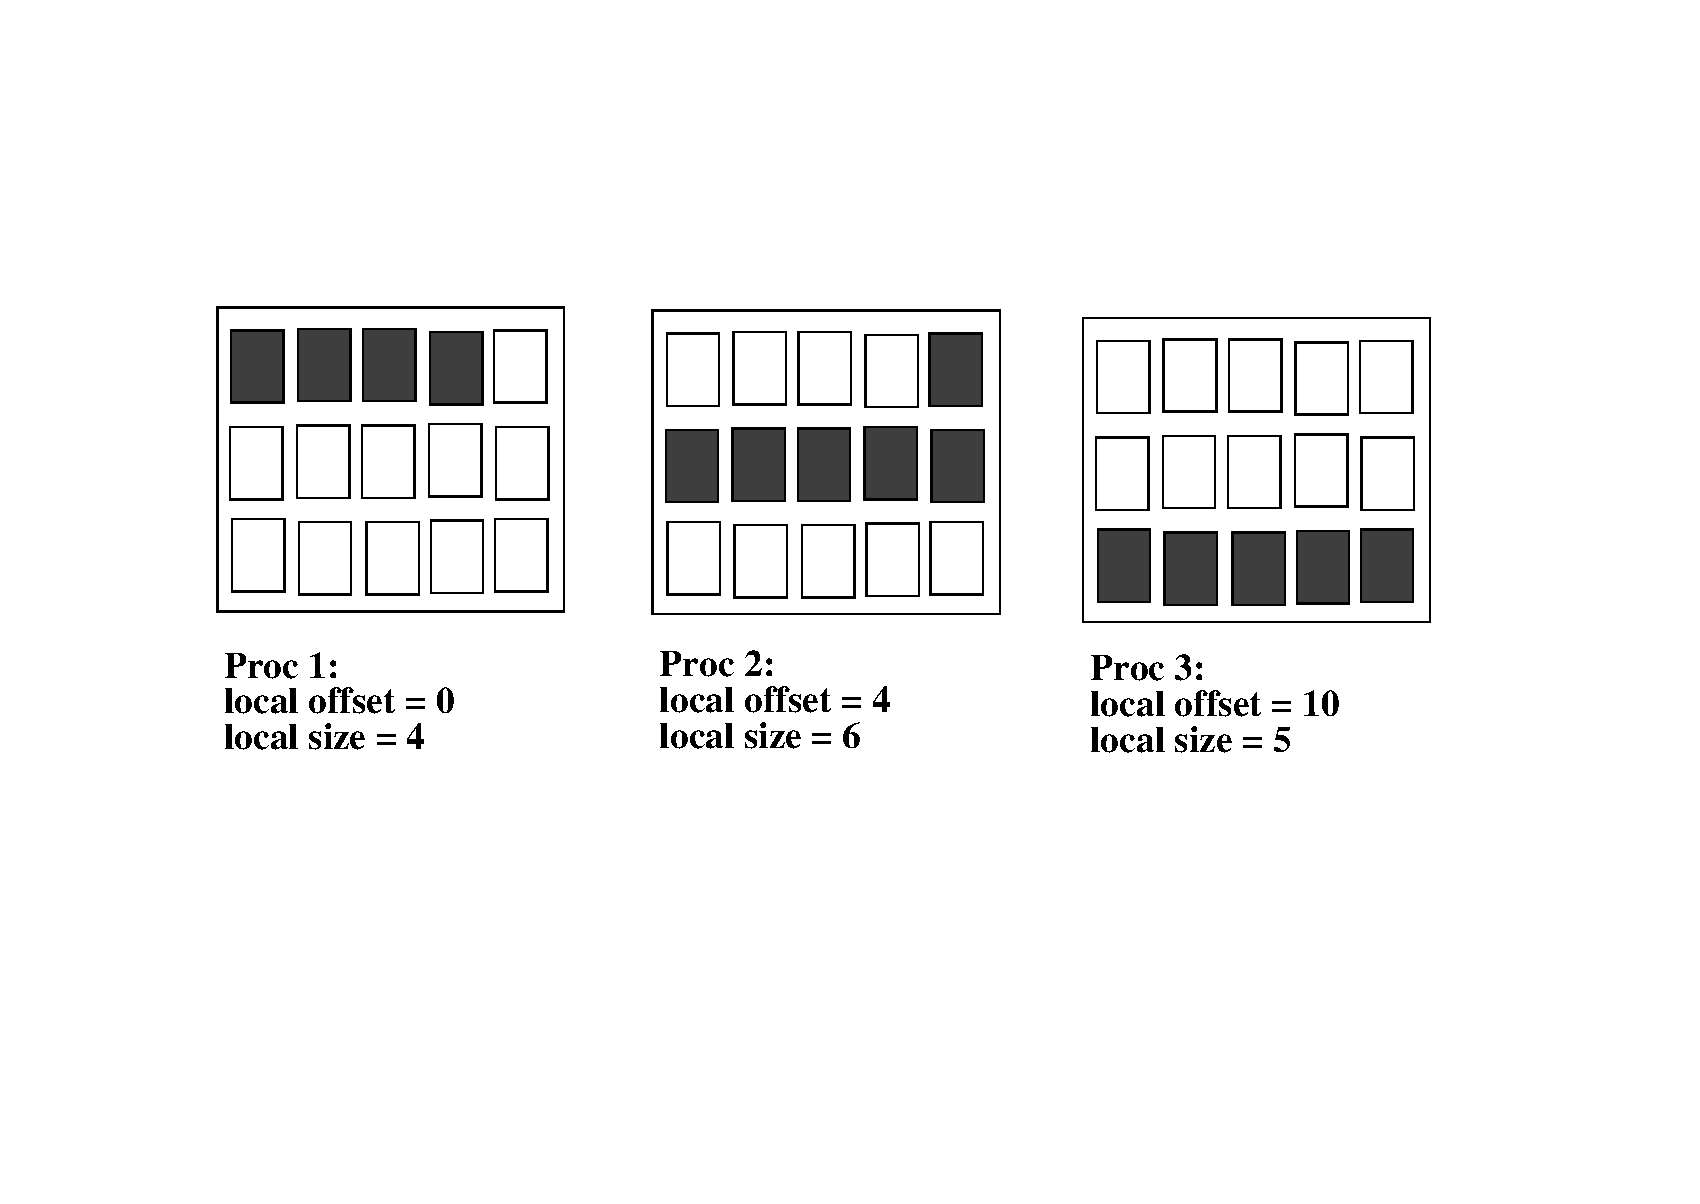
\includegraphics[scale=.6]{figures/apple_new} 
\caption{Apple partition. It is assumed here that the index start at 0 in the upper left corner.}
\label{apple_partition}
\end{figure}


\subsection{Box partition} 

Each partition is a rectangular region of the global domain, described
by the global offset of its upper left corner, and its local extents in the
X and Y dimensions. The global extent in the X dimension must also be
given. In this case, we have {\tt ig\_paral(1:5)}:
\begin{itemize}
 \item {\tt ig\_paral(1)} = 2 (indicates a Box partition)
 \item {\tt ig\_paral(2)} = the upper left corner global offset
 \item {\tt ig\_paral(3)} = the local extent in x
 \item {\tt ig\_paral(4)} = the local extent in y\footnote{The maximum
value of the local extent in y is presently 338; it can be increased
by modifying the value of {\tt Clim\_MaxSegments} in {\tt
oasis3/lib/clim/src/mod\_clim.F90} and in {\tt
oasis3/lib/psmile/src/mod\_prism\_proto.F90} and by recompiling
OASIS3 and the PSMILe library.}
 \item {\tt ig\_paral(5)} = the global extent in x.
\end{itemize}

Figure \ref{box_partition} illustrates a Box partition over 3
processes.  
 
\begin{figure}
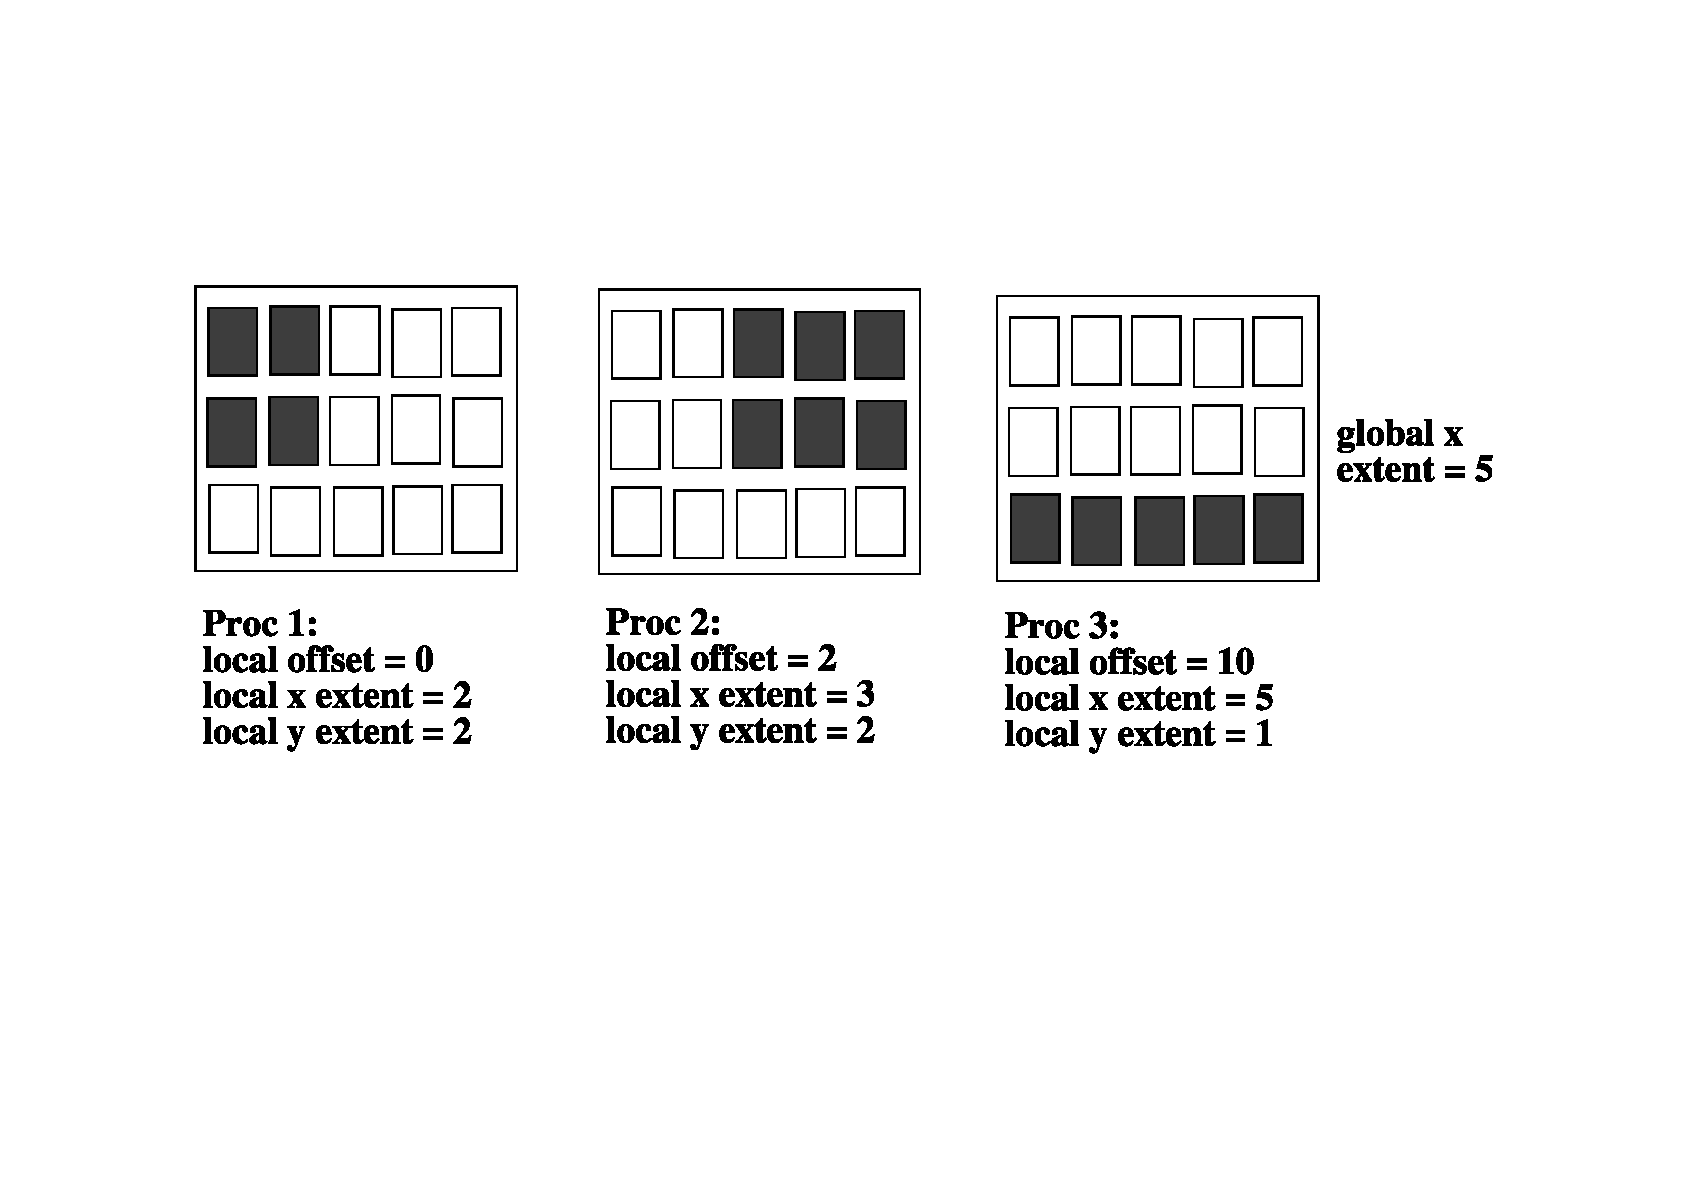
\includegraphics[scale=.6]{figures/box_new} 
\caption{Box partition. It is assumed here that the index start at 0 in the upper left corner.}
\label{box_partition}
\end{figure} 
  
\subsection{Orange partition}

{\it {\bf WARNING:} I/O do not work for Orange partition; therefore, fields having an Orange partition cannot have {\tt EXPOUT}, {\tt IGNOUT}, {\tt INPUT},{\tt OUTPUT} field status (see section \ref{subsec_namcouplesecond}).}

Each partition is an ensemble of segments of the global domain. Each
segment is described by its global offset and its local extent.  In
this case, we have {\tt ig\_paral(1:N)} where {\tt N = 2 + 2*number of
segments}\footnote{As for the Box partition, the maximum number of
segments is presently 338; it can be increased by modifying the value
of {\tt Clim\_MaxSegments}}.

\begin{itemize}
 \item {\tt ig\_paral(1)} = 3 (indicates a Orange partition)
 \item {\tt ig\_paral(2)} = the total number of segments for the partition (limited to 200 presently, see note for ig\_paral(4) for Box partition above)
 \item {\tt ig\_paral(3)} = the first segment global offset
 \item {\tt ig\_paral(4)} = the first segment local extent
 \item {\tt ig\_paral(5)} = the second segment global offset
 \item {\tt ig\_paral(6)} = the second segment local extent
 \item ...
 \item {\tt ig\_paral(N-1)} = the last segment global offset
 \item {\tt ig\_paral(N)} = the last segment local extent
\end{itemize}

Figure \ref{orange_partition} illustrates an Orange partition with 3 segments
for one process. The other process partitions are not illustrated.

\begin{figure}
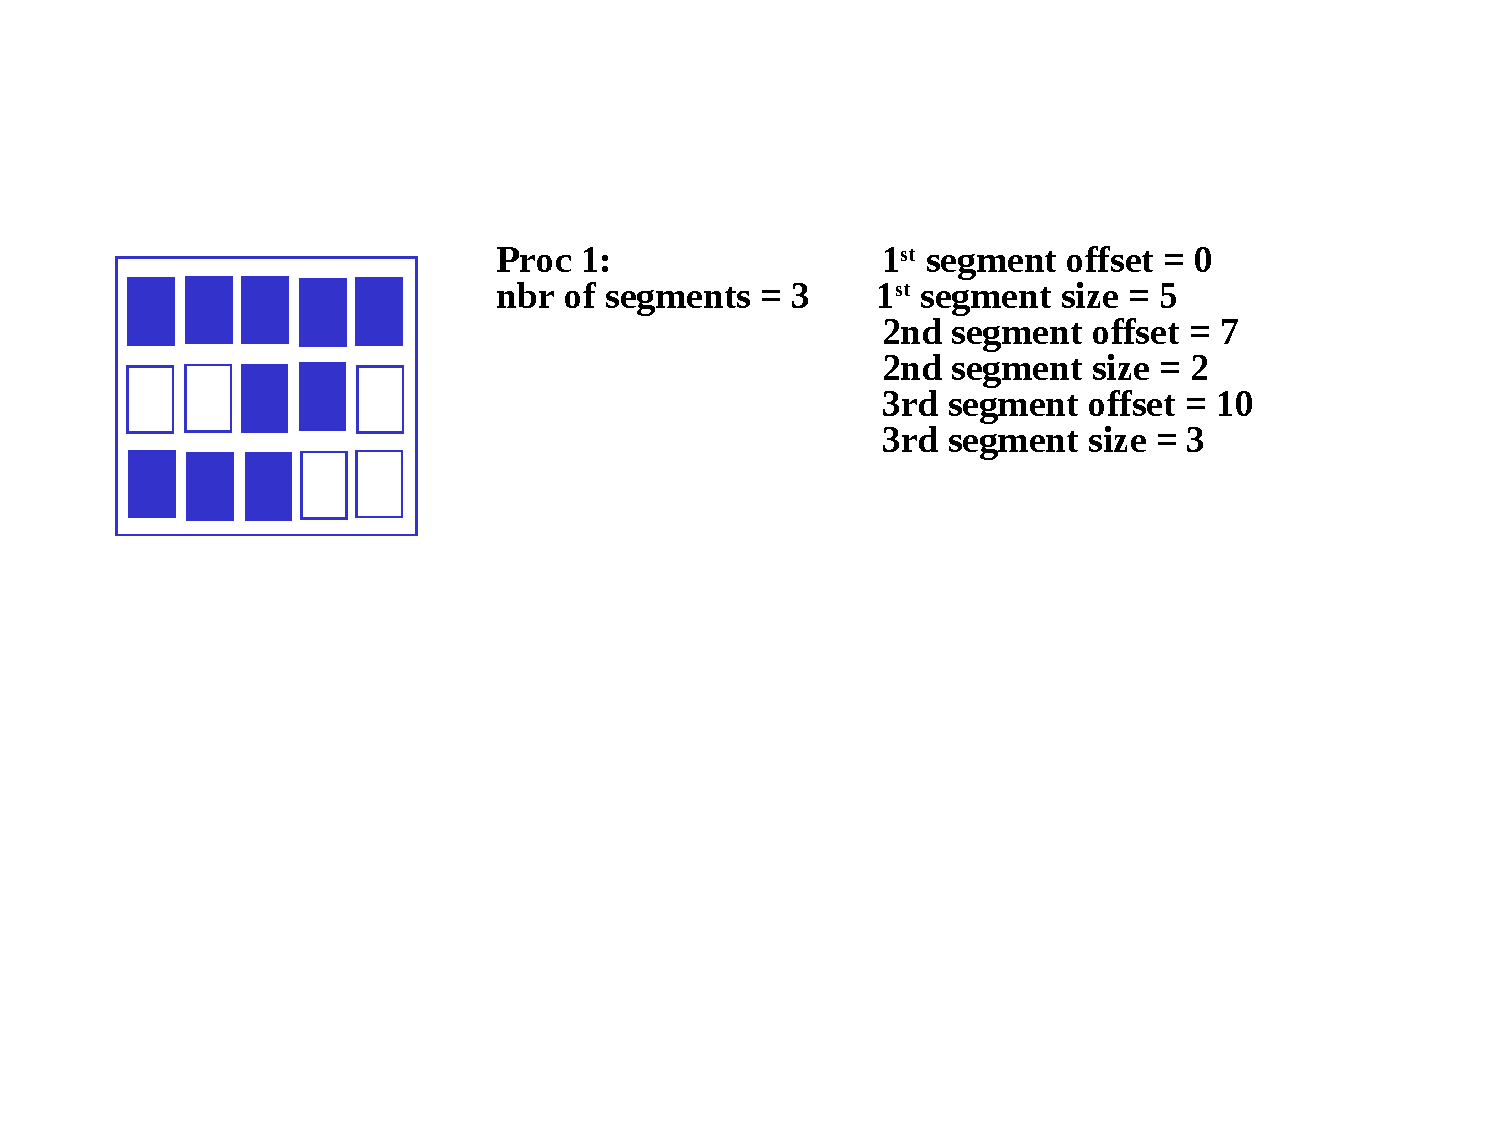
\includegraphics[scale=.6]{figures/orange_new} 
\caption{Orange partition for one process. It is assumed here that the index start at 0 in the upper left corner.}
\label{orange_partition}
\end{figure} 

%{Partition definition}

\section{I/O-coupling field declaration}
 \label{subsubsec_Declaration}

Each process exchanging coupling data declares each field it will send
or receive during the simulation. 

\begin{itemize}

\item {\tt CALL prism\_def\_var\_proto(var\_id, name, il\_part\_id,
  var\_nodims, kinout, var\_actual\_shape, var\_type, ierror)}
\item {\tt CALL oasis\_def\_var       (var\_id, name, il\_part\_id,
  var\_nodims, kinout, var\_actual\_shape, var\_type, ierror)}

\begin{itemize}
 \item {\tt var\_id [INTEGER; OUT]}: coupling field ID
 \item {\tt name [CHARACTER*8; IN]}: field symbolic name (as in the
   {\it namcouple})
 \item {\tt il\_part\_id [INTEGER; IN]}: partition ID (returned by
   {\tt prism\_def\_partition\-\_proto})
 \item {\tt var\_nodims [INTEGER, DIMENSION(2); IN]}: var\_nodims(1) is
   the rank of field array (1 or 2); var\_nodims(2) is the number of
   bundles (always 1 for OASIS3). 
 \item {\tt kinout [INTEGER; IN]}: {\tt PRISM\_In} for fields received by
   the model, or {\tt PRISM\_Out} for fields sent by the model 
 \item {\tt var\_actual\_shape [INTEGER, DIMENSION(2*var\_nodims(1)); IN]}: 
   vector of integers giving the minimum and maximum index for each
   dimension of the coupling field array; for OASIS3, the minimum
   index has to be 1 and the maximum index has to be the extent of the
   dimension.
 \item {\tt var\_type [INTEGER; IN]}: type of coupling field array;
   put {\tt PRISM\_Real} for single or double precision real
   arrays\footnote{PRISM standard is to exchange coupling fields
   declared {\tt REAL(kind=SELECTED\_REAL\_KIND(12,307))}. By default,
   all real variables are declared as such in OASIS3. To exchange
   single precision coupling fields, OASIS3 has to be compiled with
   the CPP key {\tt use\_realtype\_single}, and the coupling fields
   must be declared {\tt REAL(kind=SELECTED\_REAL\_KIND(6,37))} in the
   component models (see also chapter \ref{sec_compilationrunning}).}. 
   Note that no automatic conversion is implemented;
   therefore, all coupling fields exchanged through OASIS3 main
   process must be of same type
   % type\footnote{Coupling fields exchanged
   % directly between two component models can have a type different
   % from the ones exchanged through OASIS3 main process, as long as
   % they are single or double precision real arrays in both models.}.
 \item {\tt ierror [INTEGER; OUT]}: returned error code. 
\end{itemize}
\end{itemize}
%{I/O-coupling field declaration}

\section{End of definition phase}
\label{subsubsec_Endofdefinition}
Each process exchanging coupling data closes the definition phase.
\begin{itemize}
\item {\tt CALL prism\_enddef\_proto(ierror)}
\item {\tt CALL oasis\_enddef       (ierror)}
\begin{itemize}
  \item ierror [INTEGER; OUT]: returned error code.
\end{itemize}
\end{itemize}

%{End of definition phase}

\section{Sending and receiving actions}
\label{subsubsec_sendingreceiving}

\subsection{Sending a coupling field}
\label{prismput}

In the model time stepping loop, each process 
sends its part of the I/O or coupling field. 

\begin{itemize} 
 
\item {\tt CALL prism\_put\_proto(var\_id, date, field\_array, info)}
\item {\tt CALL oasis\_put       (var\_id, date, field\_array, info)}
\begin{itemize}
\item {\tt var\_id [INTEGER; IN]}: field ID (from
  corresponding prism\_def\_var\_proto)
\item {\tt date [INTEGER; IN]}: number of seconds in the run at the
time of the call
\item {\tt field\_array [REAL, IN]}: I/O or coupling field array 
\item {\tt info [INTEGER; OUT]}: returned info code i.e.
   \begin{itemize} 
      \item PRISM\_Sent(=4) if the field was sent to another model 
      (directly or via OASIS3 main process)
      \item PRISM\_LocTrans (=5) if the field was only used in a time
       transformation (not sent, not output)
      \item PRISM\_ToRest (=6) if the field was written to a restart file only
      \item PRISM\_Output (=7) if the field was written to an output file only
      \item PRISM\_SentOut (=8) if the field was both written to an output file
       and sent to another model (directly or via OASIS3 main process)
      \item PRISM\_ToRestOut (=9) if the field was written both to a
       restart file and to an output file.
      \item PRISM\_Ok (=0) otherwise and no error occurred.
   \end{itemize}
\end{itemize}
\end{itemize}

This routine may be called by the model at each timestep. The sending
is actually performed only if the time obtained by adding the field
lag (see \ref{subsubsec_Algoritms}) to the argument {\tt date}
corresponds to a time at which it should be activated, given the
coupling or I/O period indicated by the user in the namcouple (see
section \ref{sec_namcouple}). A field will not be sent at all if its
coupling or I/O period indicated in the {\it namcouple} is greater
than the total run time.

If a local time transformation is indicated for the field by
the user in the namcouple (INSTANT, AVERAGE, ACCUMUL, T\_MIN or T\_MAX,
see section \ref{sec_transformations}), it is automatically performed
and the resulting field is finally sent at the coupling or I/O
frequency.

For a coupling field with a positive lag (see
\ref{subsubsec_Algoritms}), the OASIS3 restart file (see section
\ref{subsec_restartdata}) is automatically written by the
last {\tt prism\_put\_proto} call of the run, if its argument {\tt date}
+ the field lag corresponds to a coupling or I/O period. To
force the writing of the field in its coupling restart file, one can
use {\tt prism\_put\_restart\_proto} (see below).

This routine can use the buffered MPI\_BSend (by default) or the
standard send MPI\_Send (if {\tt NOBSEND} is specified in the
namcouple -see {\tt \$CHANNEL} section
\ref{subsec_namcouplefirst}) to send the coupling fields.

\vspace*{0.5cm}

\subsection{Receiving a coupling field}

\vspace*{0.5cm}

In the model time stepping loop, each process
receives its part of the I/O-coupling field. 

\begin{itemize} 

\item {\tt CALL prism\_get\_proto(var\_id, date, field\_array, ierror)}
\item {\tt CALL oasis\_get       (var\_id, date, field\_array, ierror)}
\begin{itemize}
\item {\tt var\_id [INTEGER; IN]}: field ID (from
  corresponding prism\_def\_var\_proto)
\item {\tt date [INTEGER; IN]}: number of seconds in the run at the
time of the call
\item {\tt field\_array [REAL, OUT]}: I/O or coupling field array 
\item {\tt info [INTEGER; OUT]}: returned info code
   \begin{itemize} 
      \item PRISM\_Recvd(=3) if the field was received from another model
       (directly or via OASIS3 main process)
      \item PRISM\_FromRest (=10) if the field was read from a restart
       file only (directly or via OASIS3 main process)
      \item PRISM\_Input (=11) if the field was read from an input
       file only
      \item PRISM\_RecvOut (=12) if the field was both received from
       another model (directly or via OASIS3 main process) and written to
       an output file
      \item PRISM\_FromRestOut (=13) if the field was both read from a
       restart file (directly or via OASIS3 main process) and written to an
       output file
      \item PRISM\_Ok (=0) otherwise and no error occurred.
   \end{itemize}
\end{itemize}
\end{itemize}

This routine may be called by the model at each timestep. The {\tt date}
argument is automatically analysed and the receiving action is actually
performed only if {\tt date} corresponds to a time for which it should
be activated, given the period indicated by the user in the
namcouple. A field will not be received at all if its
coupling or I/O period indicated in the {\it namcouple} is greater
than the total run time.

\subsection{Auxiliary routines}
\label{subsec:auxiliary}

Auxiliary routines available in oasis3 are not yet available.

\begin{itemize} 
\item {\tt CALL prism\_get\_debug(debug\_value)}
\item {\tt CALL oasis\_get\_debug(debug\_value)}
\begin{itemize}
\item {\tt debug\_value [INTEGER; OUT]}: debug value
\end{itemize}
\end{itemize}

This routine may be called at any time to retrieve the current
debug level internal to oasis.  This is useful if changing debug
levels and the user wants to return the debug value later to
its prior value, or if a user wants to key off the oasis
debug level for model debug diagnostics.


\begin{itemize} 
\item {\tt CALL prism\_set\_debug(debug\_value)}
\item {\tt CALL oasis\_set\_debug(debug\_value)}
\begin{itemize}
\item {\tt debug\_value [INTEGER; IN]}: debug value
\end{itemize}
\end{itemize}

This routine may be called at any time to change the debug level in oasis.
The debug level is initially set for all processors and all models
by the NLOGPRT namcouple input.  This method allows users to vary 
the debug level by model, task, or at different points in the model
integration.


%\begin{itemize} 
%\item {\tt CALL prism\_put\_inquire(var\_id, date, info)}
%\begin{itemize}
%\item {\tt var\_id [INTEGER; IN]}: field ID (from
%  corresponding prism\_def\_var\_proto)
%\item {\tt date [INTEGER; IN]}: number of seconds in the run at the
%time of the call
%\item {\tt info [INTEGER; OUT]}: returned info code. 
%\end{itemize}
%\end{itemize}
%
%This routine may be called at any time to
%inquire what would happen to the corresponding field (i.e. with same
%{\tt var\_id} and at same {\tt date}) below the corresponding {\tt
%  prism\_put\_proto}. The possible value of the returned info code are
%as for {\tt prism\_put\_proto}:   
%\begin{itemize}
%      \item PRISM\_Sent(=4) if the field would be sent to another model 
%      (directly or via OASIS3 main process)
%      \item PRISM\_LocTrans (=5) if the field would be only used in a time
%       transformation (not sent, not output)
%      \item PRISM\_ToRest (=6) if the field would be written to a restart file only
%      \item PRISM\_Output (=7) if the field would be written to an output file only
%      \item PRISM\_SentOut (=8) if the field would be both written to an output file
%       and sent to another model (directly or via OASIS3 main process)
%      \item PRISM\_ToRestOut (=9) if the field would be written both to a
%       restart file and to an output file.
%      \item PRISM\_Ok (=0) otherwise and no error occurred. 
%\end{itemize}
%This is useful when the
%calculation of the corresponding {\tt field\_array} is CPU consuming
%and should be avoided if the field is not effectively used below the {\tt
%prism\_put\_proto}.
%
%\begin{itemize} 
%\item {\tt CALL prism\_put\_restart\_proto(var\_id, date, ierror)}
%\begin{itemize}
%\item {\tt var\_id [INTEGER; IN]}: field ID (from
%  corresponding prism\_def\_var\_proto)
%\item {\tt date [INTEGER; IN]}: number of seconds in the run at the
%time of the call
%\item {\tt info [INTEGER; OUT]}: returned error code (should be
%  PRISM\_ToRest=6 if the restart writing was successful)
%\end{itemize}
%\end{itemize}
%
%This routine forces the writing of the field with corresponding {\tt
%var\_id} in its coupling restart file (see section
%\ref{subsec_restartdata}). If a time operation is specified for this
%field, the value of the field as calculated below the last {\tt
%prism\_put\_proto} is written. If no time operation is specified, the
%value of the field transferred to the last {\tt prism\_put\_proto} is
%written.
%
%%{sending and receiving actions}
%
%\begin{itemize} 
%\item {\tt CALL prism\_get\_freq (var\_id, period, ierror)}
%\begin{itemize}
%\item {\tt var\_id [INTEGER; IN]}: field ID (from
%  corresponding prism\_def\_var\_proto)
%\item {\tt period [INTEGER; OUT]}: period of coupling (in number of seconds)
%\item {\tt ierror [INTEGER; OUT]}: returned error code
%\end{itemize}
%\end{itemize}
%This routine can be used to retrieve the coupling period of field with
%corresponding {\tt var\_id}, as defined in the {\it namcouple} (see
%also section \ref{subsubsec_secondEXPORTED}).

\section{Termination}
\label{subsubsec_Termination}

\begin{itemize}

\item {\tt CALL prism\_terminate\_proto(ierror)}
\item {\tt CALL oasis\_terminate       (ierror)}
  \begin{itemize}
  \item {\tt ierror [INTEGER; OUT]}: returned error code.
  \end{itemize}
  All processes of the component model must terminate the coupling by calling {\tt
  prism\_terminate\_proto}\footnote{If the process called {\tt
  MPI\_Init} (before calling {\tt prism\_init\_comp\_proto}), it must
  also call {\tt MPI\_Finalize} explicitly, but only after calling
  {\tt prism\_terminate\_proto}.} (normal termination). OASIS3 will
  terminate after all processes called
  prism\_terminate\_proto. With MPI2, the run may be considered
  finished when OASIS3 terminates; to avoid problem, place the call
  to prism\_terminate\_proto at the very end in the component model code.

\item {\tt CALL prism\_abort\_proto(compid, routine\_name, abort\_message)}
\item {\tt CALL oasis\_abort       (compid, routine\_name, abort\_message)}
\begin{itemize}
  \item {\tt compid [INTEGER; IN]}: component model ID (from
prism\_init\_comp\_proto) 
  \item {\tt routine\_name; IN]}: name of calling routine
  \item {\tt abort\_message; IN]}: message to be written out.
\end{itemize}

 If a process needs to abort voluntarily, it should do so by
 calling {\tt prism\_abort\_proto}. This will ensure a proper
 termination of all processes in the coupled model communicator. This
 routine writes the name of the calling model, the name of the
 calling routine, and the message to the job standard output (stdout). 
 This routine cannot be called before {\tt prism\_init\_comp\_proto}.

\end{itemize}

%{Termination}

\section{Coupling algorithms - SEQ and LAG concepts}
\label{subsubsec_Algoritms}

Using the PSMILe library, the user has full flexibility to reproduce
different coupling algorithms. In the component codes, the sending and
receiving routines, respectively {\tt prism\_put\_proto} and {\tt
  prism\_get\_proto}, can be called at each model timestep, with the
appropriate {\tt date} argument giving the actual time (at the
beginning of the timestep), expressed in ``number of seconds since the
start of the run''. This {\tt date} argument is automatically analysed
by the PSMILe
%\footnote{With the PIPE, SIPC, GMEM and previously with
%the CLIM communication techniques, no such analysis was performed. For
%PIPE, SIPC, and GMEM, the sending actions on the source side would
%automatically match the receiving actions on the target side on a FIFO
%(First In First Out) basis.} 
and depending on the coupling period and the lag (LAG) chosen by the 
user for each coupling field in the configuration file {\it namcouple}, different
coupling algorithms can be reproduced without modifying anything in the
component model codes themselves. 

The lag (LAG) value tells the coupler to modify the time that data
is sent (put) by the amount of the lag.  The lag can be positive or
negative but should never be larger (in absolute magnitude) than the
coupling period of any field due to problems with restart-ability and
dead-locking.  A positive lag indicates the
put will occur sooner than zero lag and a negative lag tells the coupler
to send the data later than zero lag.  When the lag is positive, 
a restart file must be available to initiate the coupling and in those cases, 
the restart file is then updated at the end of the run.  A positive
lag acts like a send occurred before the model started.  To mimic that
mode, the restart data is sent at time=0, the two models then couple at the coupling
period with the given lag on the send side, and then the final coupling
data on the source side is written to the restart file for use in the
next run.  

The order of coupling operations is the system is now determined solely
by the order of calls to send (put) and receive (get) data in the models
in conjunction with the setting of the lag in the namcouple.  Data that is
received (get) is always blocking while data that is sent (put) is non-blocking
with respect to the model making that call.  It is possible
to deadlock the system if the relative order of puts and gets in different
models is not compatable.  The SEQ index is no longer needed in the namcouple
input to specify the sequencing order of different coupling fields.
The sequence (SEQ) index in the namcouple file now provides the coupling 
layer with an ability to detect a deadlock before it happens and exit 
gracefully.  It does this by tracking the order of get and put calls in
models compared to the SEQ specified in the namcouple.  If there are any
inconsistencies, the model will abort gracefully with a useable error
message before the system deadlocks.  If there are any coupling dependencies
in the system, use of the SEQ index is recommended for diagnosis, but again,
it has no impact on the ultimate solution.

The lag concept and indices are explained in more detail below and some
examples are provided.

\subsection{The lag concept}
\label{subsub_lag}

If no lag index or if a lag index equal to 0 is given by the user in
the {\it namcouple} for a particular coupling field, the sending or
receiving actions will actually be performed, below the {\tt
  prism\_put\_proto} called in the source model or below the {\tt
  prism\_get\_proto} called in the target model respectively, each time the
{\tt date} argument on both sides matches an integer number of
coupling periods.
 
\vspace*{0.5cm}

To match a {\tt prism\_put\_proto} called by the source model at a
particular {\tt date} with a {\tt prism\_get\_proto} called by the target
model at a different {\tt date}, the user has to define in the {\it
namcouple} an appropriate lag index, LAG, for the coupling field(see
section \ref{sec_namcouple}). The value of the LAG index must be
expressed in ``number of seconds''; its value is automatically added
to the {\tt prism\_put\_proto} {\tt date} value and the sending action is
effectively performed when the sum of the {\tt date} and the lag matches an
integer number of coupling periods. The lag can be positive or negative,
but it must never be greater than the coupler period or less than or
equal to the (-) coupling period.  This sending action is
automatically matched, on the target side, with the receiving action
performed when the {\tt prism\_get\_proto date} argument equals the
same integer number of coupling periods.  The lag only shifts the
time data is sent.  It cannot be used to shift the time data is
received yet.

Note that when there is a lag, the first instance of the source field
is missing in the debug file (EXPOUT or IGNOUT fields, see section
\ref{subsec_namcouplesecond}) because the first source field is not
sent by the source model with a {\tt prism\_put\_proto} but directly
read by OASIS3 from a coupling restart file.
 
  \begin{enumerate}

  \item LAG concept first example
 
  A first coupling algorithm, exploiting the LAG concept, is
  illustrated on figure \ref{fig:lag_concept_1}. 


  On the 4 figures in this section, short black arrows correspond to {\tt
  prism\_put\_proto} or \break {\tt prism\_get\_proto} called in the component model
  that do not lead to any sending or receiving action;
  long black arrows correspond to {\tt prism\_put\_proto} or {\tt
  prism\_get\_proto} called in the component models that do
  effectively lead to a sending or receiving action;
  long red arrows correspond to {\tt prism\_put\_proto} or {\tt
  prism\_get\_proto} called in the component models that lead to a
  reading or writing of the coupling field from or to a coupling
  restart file (either directly or through OASIS3 main process).

\begin{figure}
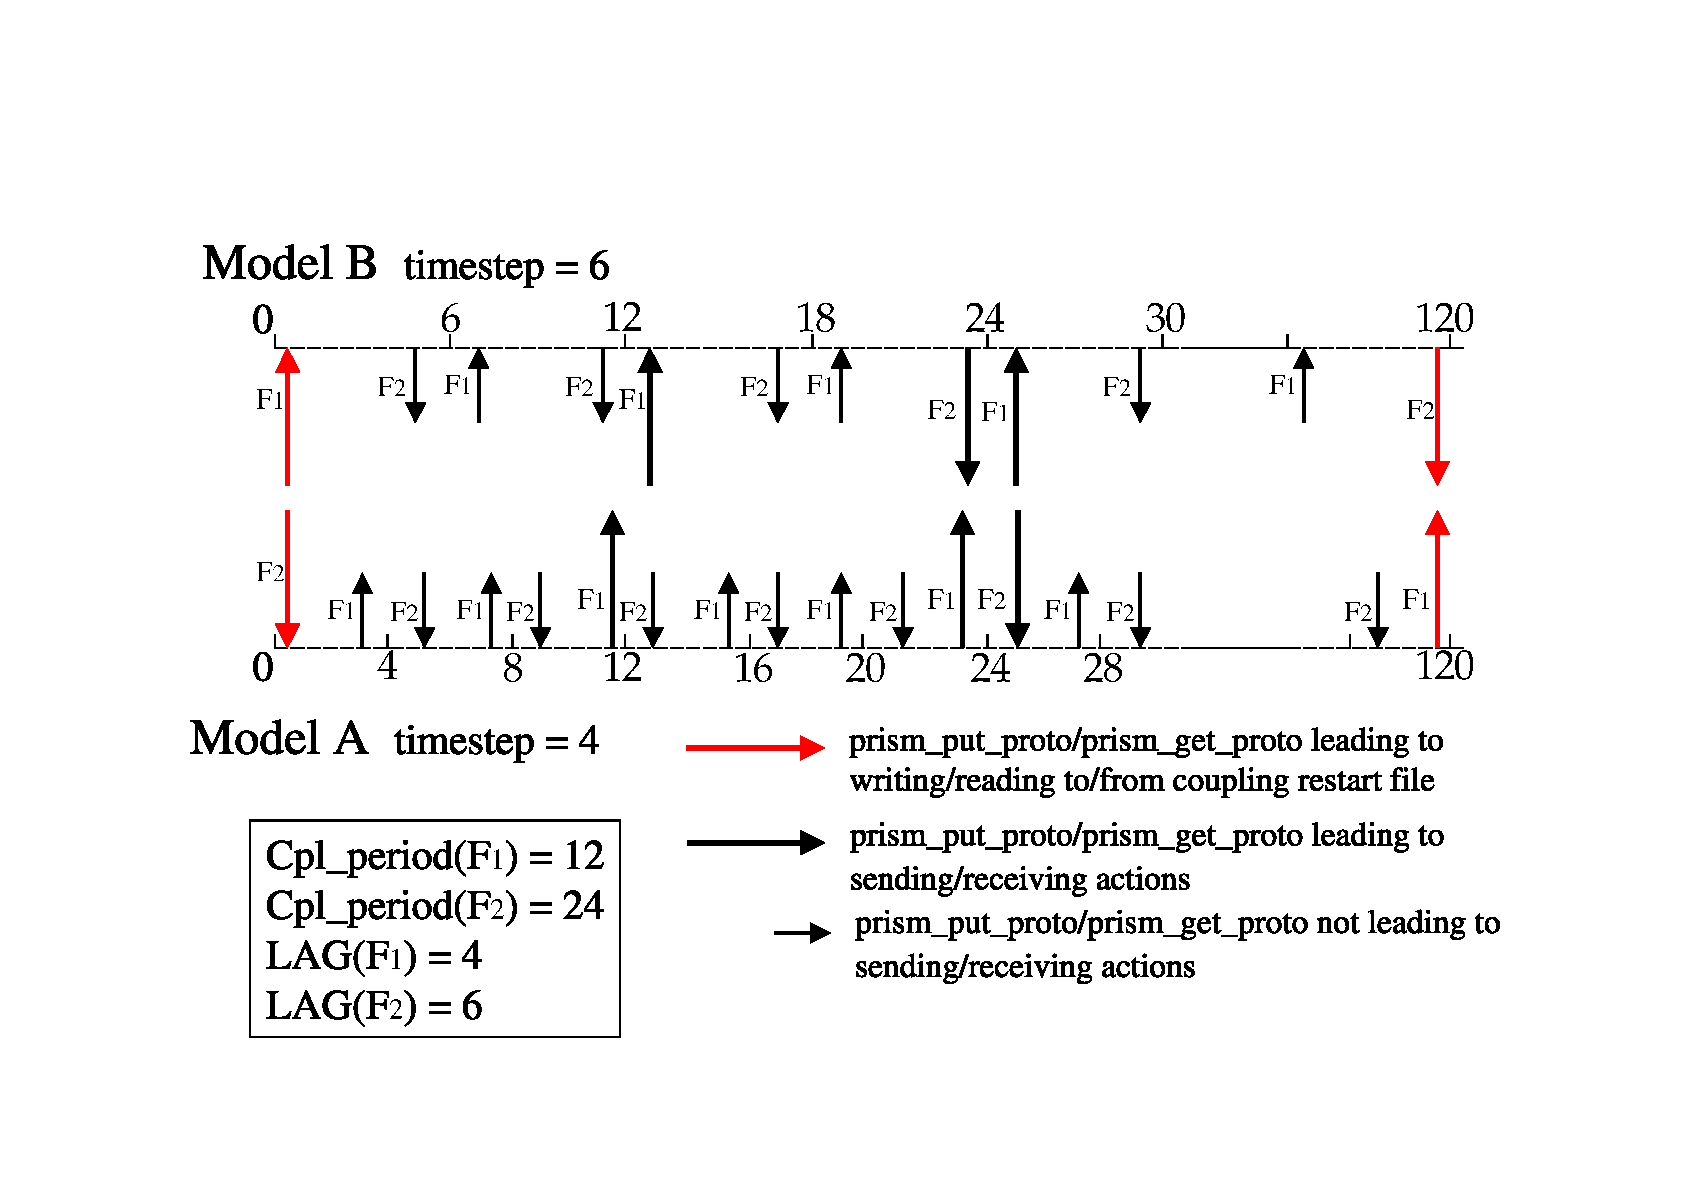
\includegraphics[scale=.6]{figures/fig_lag_concept_1}
\caption{LAG concept first example} 
\label{fig:lag_concept_1}
\end{figure}

  During a coupling timestep, model A receives $F_2$ and then sends $F_1$; its
  timestep length is 4. During a coupling timestep, model B receives $F_1$
  and then sends $F_2$; its timestep length is 6.  $F_1$ and $F_2$
  coupling periods are respectively 12 and 24. If $F_1$/$F_2$ sending
  action by model A/B was used at a coupling timestep to match the
  model B/A receiving action, a deadlock would occur as both models
  would be initially waiting on a receiving action. To prevent this,
  $F_1$ and $F_2$ produced at the timestep before have to be used to
  match respectively the model B and model A receiving actions.

  This implies that a lag of respectively 4 and 6 seconds must be
  defined for $F_1$ and $F_2$. For $F_1$, the {\tt prism\_put\_proto}
  performed at time 8 and 20 by model A will then lead to sending actions
  (as 8 + 4 = 12 and 20 + 4 = 24 which are coupling periods) that
  match the receiving actions performed at times 12 and 24 below the {\tt
  prism\_get\_proto} called by model B.  For $F_2$, the {\tt
  prism\_put\_proto} performed at time 18 by model B then leads to
  a sending action (as 18 + 6 = 24 which is a coupling
  period) that matches the receiving action performed at time 24
  below the {\tt prism\_get\_proto} called by model A.

  At the beginning of the run, as their LAG index is greater than 0,
  the first {\tt prism\_get\_proto} of $F_1$ and $F_2$ will automatically 
  be fulfilled by OASIS3 with fields read from their respective coupling restart files. The user
  therefore has to create those coupling restart files before the first
  run in the experiment. At the end of the run, $F_1$
  having a lag greater than 0, is automatically written to its
  coupling restart file below the last $F_1$ {\tt prism\_put\_proto} as the
  {\tt date} + $F_1$ lag equals a coupling time. The analogue is true
  for $F_2$. These
  values will automatically be read in at the beginning of the next
  run below the respective {\tt prism\_get\_proto}.

  \item LAG concept second example

  A second coupling algorithm exploiting the LAG concept is
  illustrated on figure \ref{fig:lag_concept_2}. During its timestep,
  model A receives $F_2$, sends $F_3$ and then $F_1$; its timestep
  length is 6. During its timestep, model B receives $F_1$, receives
  $F_3$ and then sends $F_2$; its timestep length is also 6.  $F_1$,
  $F_2$ and $F_3$ coupling periods are both supposed to be equal to
  12.
 
\begin{figure}
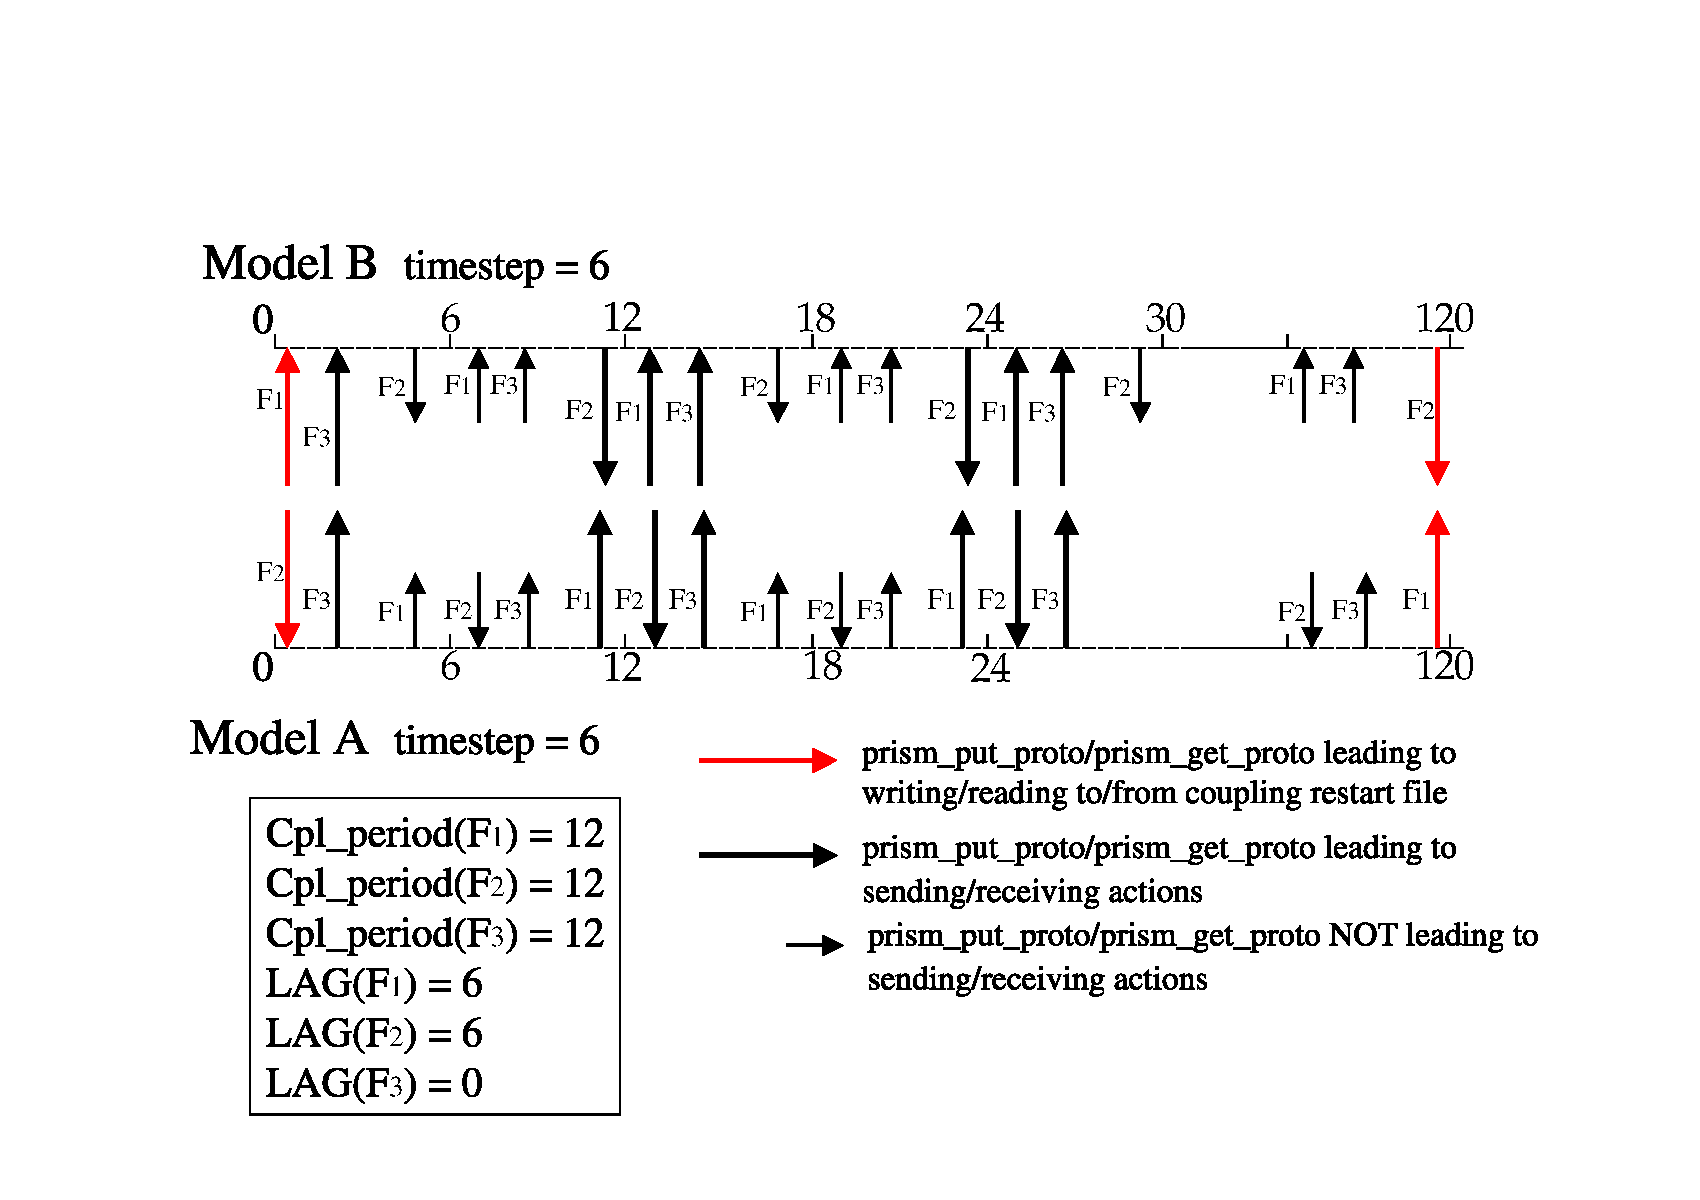
\includegraphics[scale=.6]{figures/fig_lag_concept_2} 
\caption{LAG concept second example} 
\label{fig:lag_concept_2}
\end{figure}

  For $F_1$ and $F_2$ the situation is similar to the first
  example. If $F_1$/$F_2$ sending action by model A/B was used at a
  coupling timestep to match the model B/A receiving action, a
  deadlock would occur as both models would be waiting on a receiving
  action. To prevent this, $F_1$ and $F_2$ produced at the timestep
  before have to be used to match the model A and model B receiving
  actions, which means that a lag of 6 must be defined for both $F_1$
  and $F_2$. For both coupling fields, the {\tt prism\_put\_proto}
  performed at times 6 and 18 by the source model then lead to sending
  actions (as 6 + 6 = 12 and 18 + 6 = 24 which are coupling periods)
  that match the receiving action performed at time 12 and 24 below
  the {\tt prism\_get\_proto} called by the target model.

  For $F_3$, sent by model A and received by model B, no lag
  needs to be defined: the coupling field produced by model A at the
  coupling timestep can be ``consumed'' by model B without causing a
  deadlock situation.

  As in the first example, the {\tt prism\_get\_proto} performed at
  the beginning of the run for $F_1$ and $F_2$, automatically read
  them from their coupling restart files, and the last {\tt
  prism\_put\_proto} performed at the end of the run automatically
  write them to their coupling restart file. For $F_3$, no coupling
  restart file is needed nor used as at each coupling period the
  coupling field produced by model A can be directly ``consumed'' by
  model B.

  We see here how the introduction of appropriate LAG indices results in
  receiving in the target model,
  coupling fields produced by the
  source model the timestep before; this is, in some coupling
  configurations, essential to avoid deadlock situations.

  \end{enumerate}

\subsection{The sequence concept}

*** Add some new description and examples ***
 
%To exchange the coupling fields going through OASIS3 main process
%(i.e. with status EXPORTED, AU-\newline XILARY, or EXPOUT, see section
%\ref{sec_namcouple}), in a given order at each coupling timestep, a
%sequence index SEQ must be defined for each of them. This is not
%required for I/O fields or for coupling fields exchanged directly
%between the component models, i.e. with status IGNOUT, INPUT or
%OUTPUT. SEQ gives the position of the coupling field in the
%sequence.
%
%
%\begin{figure}
%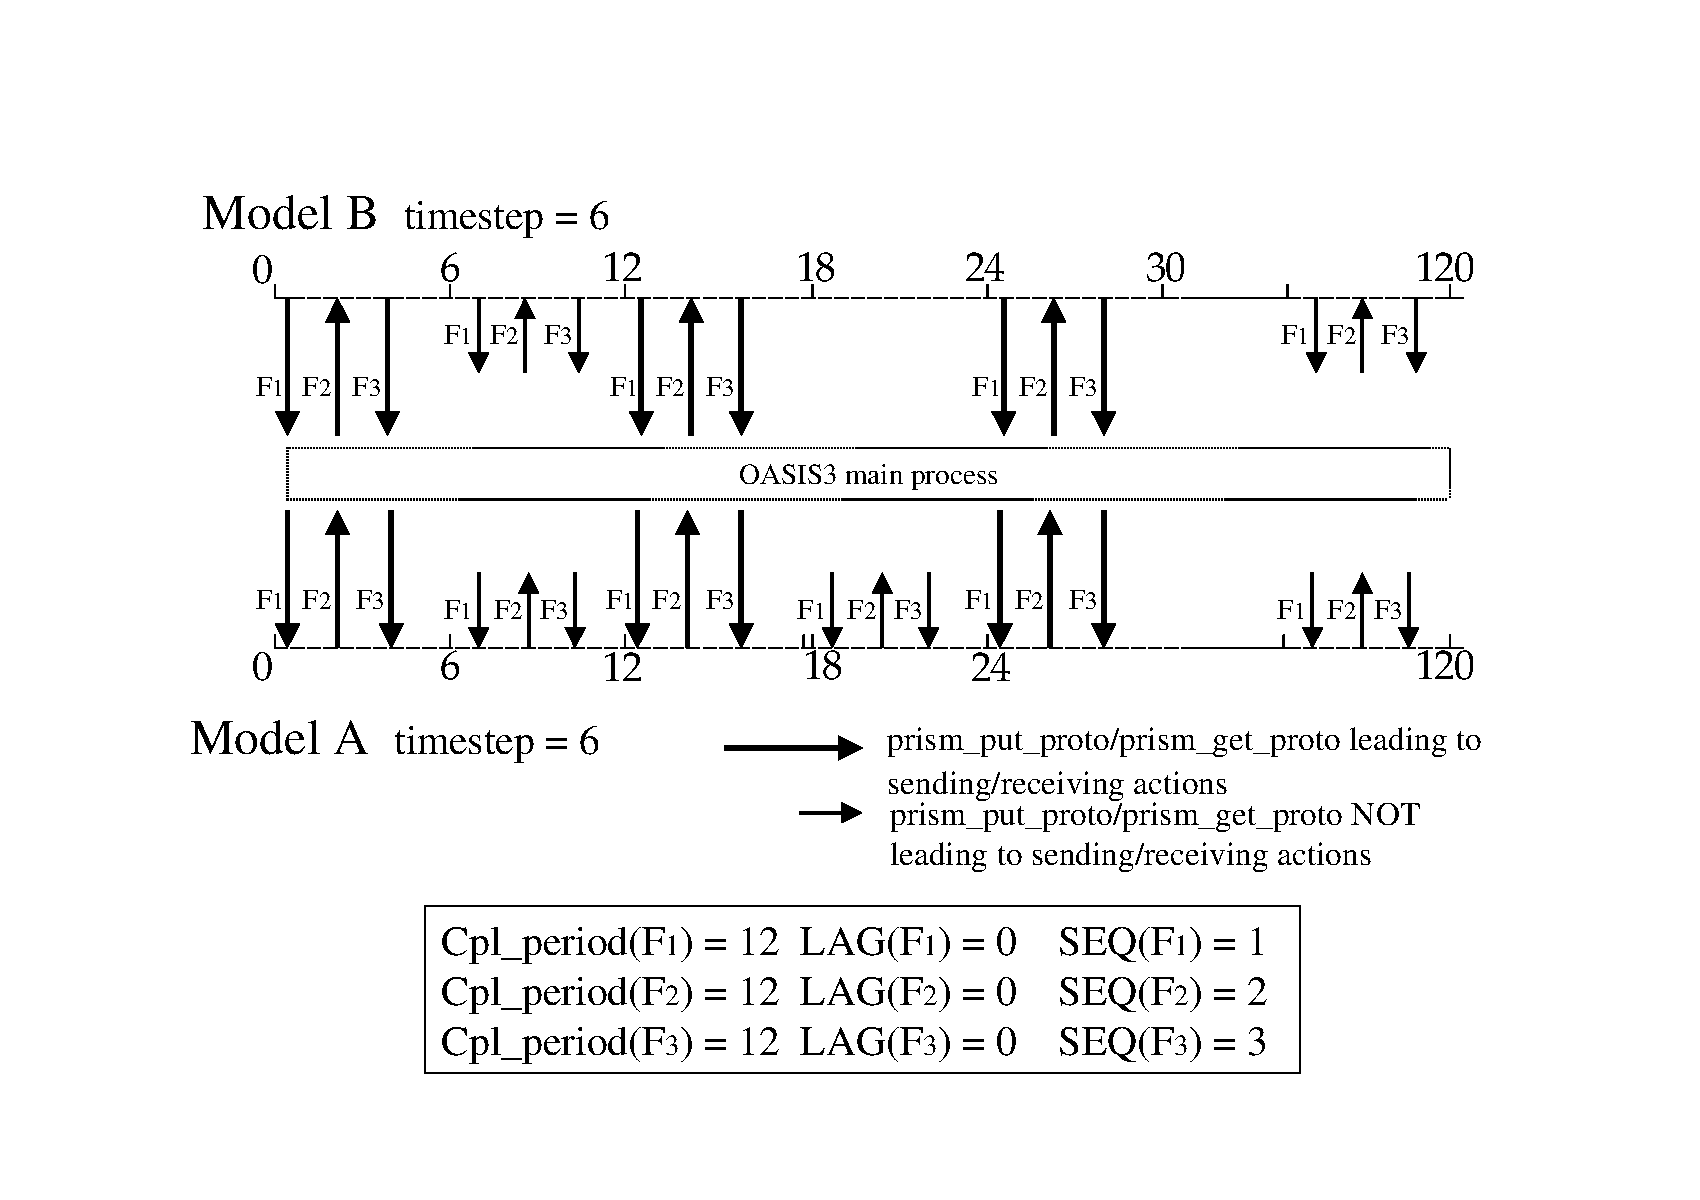
\includegraphics[scale=.6]{figures/fig_seq_concept} 
%\caption{The SEQ concept}
%\label{fig:seq_concept}
%\end{figure}
%
%A coupling algorithm, showing the SEQ concept, is illustrated on
%figure \ref{fig:seq_concept}. All coupling field produced by the
%source model at the coupling timestep can be ``consumed'' by the
%target model at the same timestep without causing any
%deadlock situation; therefore, LAG = 0 for all coupling fields.
%However, at each coupling timestep, a particular order
%of exchange must be respected; $F_1$ must be received by
%model A before it can send $F_2$, which in turn must be received by model B
%before it can send $F_3$. Therefore, SEQ = 1, 2, 3 must be defined
%respectively for $F_1$, $F_2$ and $F_3$. 
%As all fields can be consumed at the time they are produced (LAG=0 for
%all fields), there no reading/writing from/to coupling restart files.
%
%An appropriate use of the SEQ index can optimise a coupled run when 
%one of the component model is much slower than the other. This is illustrated 
%on figure \ref{fig:seq_optim}.
% \begin{figure}
%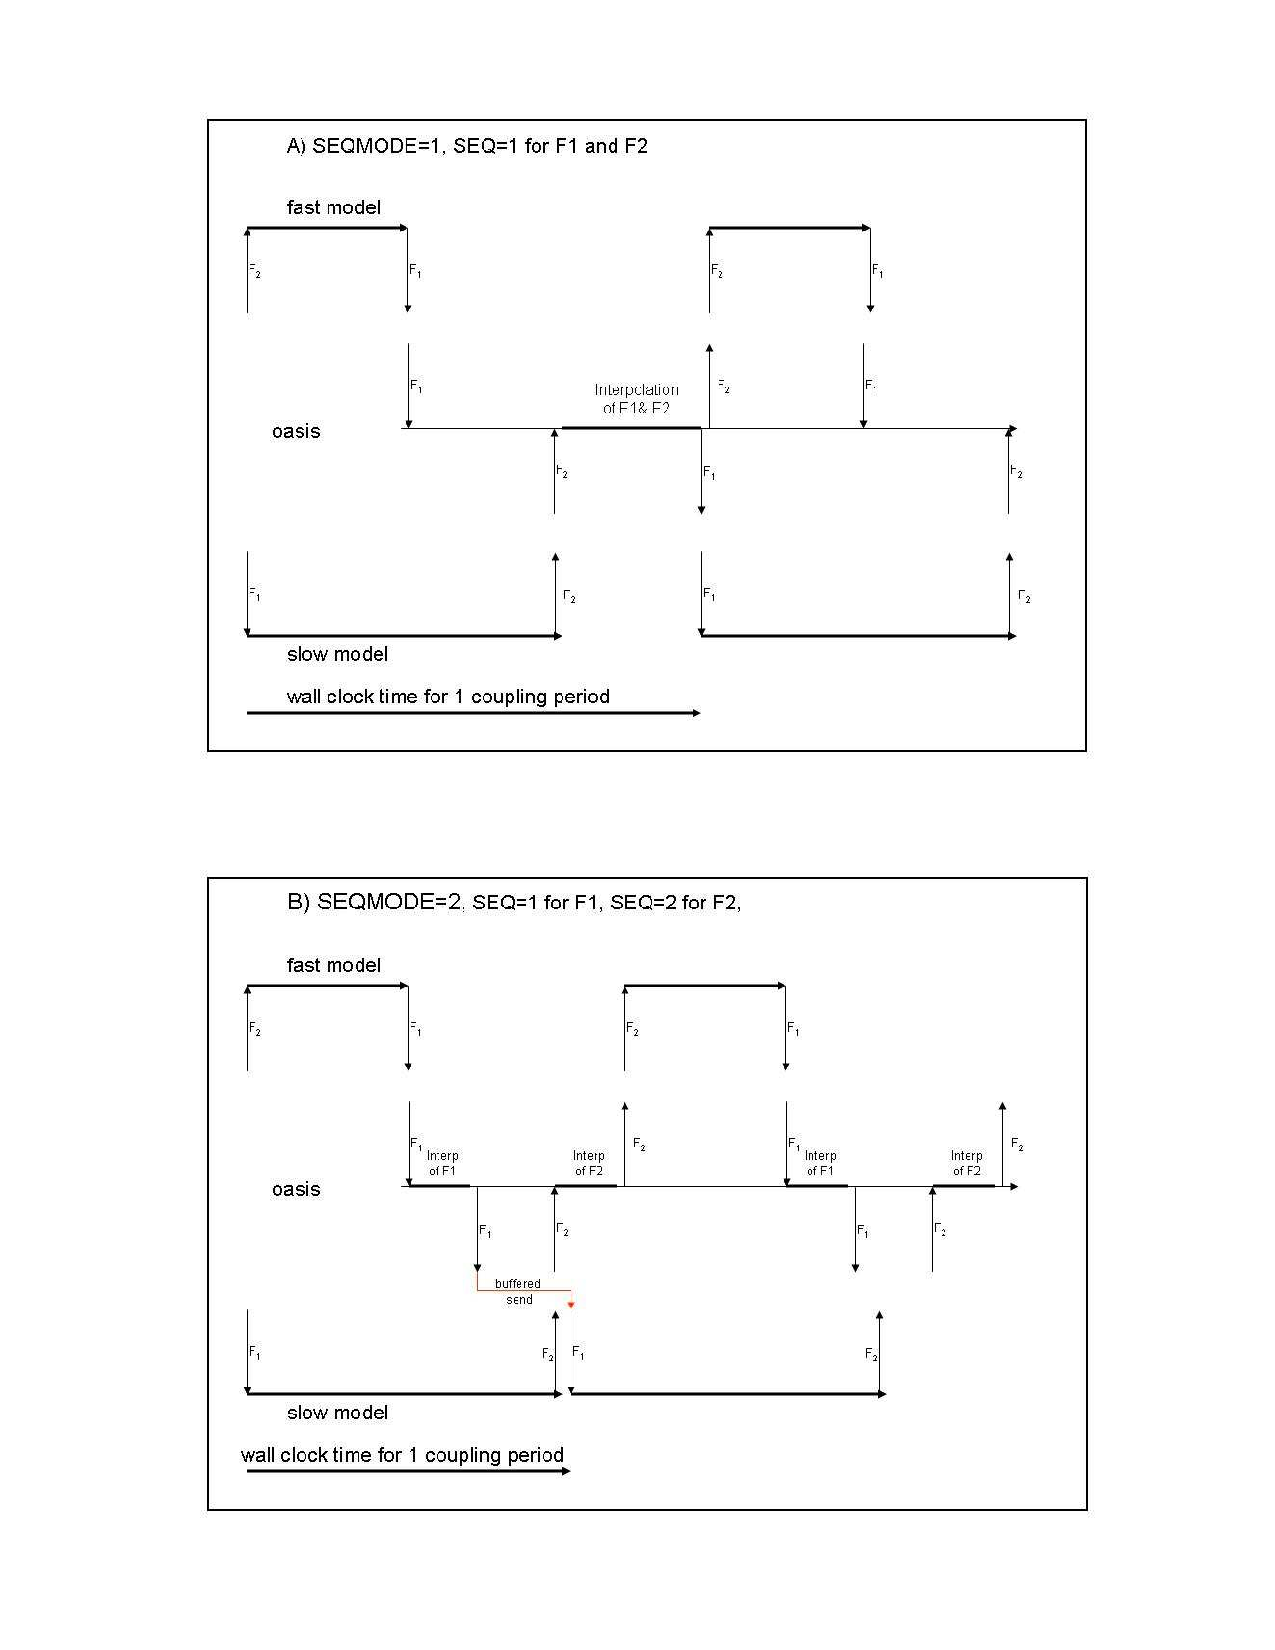
\includegraphics[scale=.6]{figures/fig_seq_optim} 
%\caption{Optimisation of a coupled run using the SEQ index}
%\label{fig:seq_optim}
%\end{figure}
%
%In part A of figure \ref{fig:seq_optim} , a coupled run with no use of the SEQ
%index is illustrated.  When the fast model reaches a coupling period,
%it sends its output coupling fields to OASIS that receives them and
%then waits until the slow model has also reaches the coupling period.
%Once OASIS3 has received the fields from both the fast and the slow
%components, it transforms them and send them respectively to the slow
%and the fast components. Only then the fast and the slow components
%are able to go on. The total elapse time for a coupling period is the
%sum of the slow model running time and the OASIS3 working time.  
%
%In part B of figure \ref{fig:seq_optim}, an index SEQ = 1 is assigned to the
%coupling fields going from the fast to the slow component and an index
%SEQ = 2 is assigned to the coupling fields going from the slow to the
%fast component. When the fast model reaches a coupling period, it
%sends its output coupling fields to OASIS3 that receives them, treats
%them and sends them to the slow model.  As soon as the slow model also
%reaches the coupling period, it sends its output coupling fields to
%OASIS, receives its input coupling fields right after, and is then
%able to go on without any delay.  Concurrently, OASIS3 treats the slow
%model output component fields and sends them to the fast model that is
%then able to go on. Here the total elapse time for a coupling period
%is very close to the slow model running time only. One can see that
%using the SEQ index in this way results in ``hiding'' OASIS3 working
%time behind the slow model running time. Note that in this case, the
%default buffered send must be used (i.e the {\tt NOBSEND} option
%cannot be specified in the {\it namcouple}, see section
%\ref{subsec_namcouplefirst}).
%
%\subsection{A mix of lag and sequence: the sequential coupled model}
%\label{subsubsec_mix}
%
%One can run the same component models simultaneously or sequentially
%by defining the appropriate LAG and SEQ indices. In the example
%illustrated on figure \ref{fig:mix_seqlag}, the models perform their
%{\tt prism\_put\_proto} and {\tt prism\_get\_proto} calls exactly as
%in the first lag example above (see 1. of \ref{subsub_lag}): model A receives $F_2$ and then sends
%$F_1$; its timestep length is 4. During a coupling timestep, model B
%receives $F_1$ and then sends $F_2$; its timestep length is 6.  $F_1$
%and $F_2$ coupling periods are both 12. By defining a LAG index of -8
%for $F_1$, the models will now run sequentially.
%
%\begin{figure}
%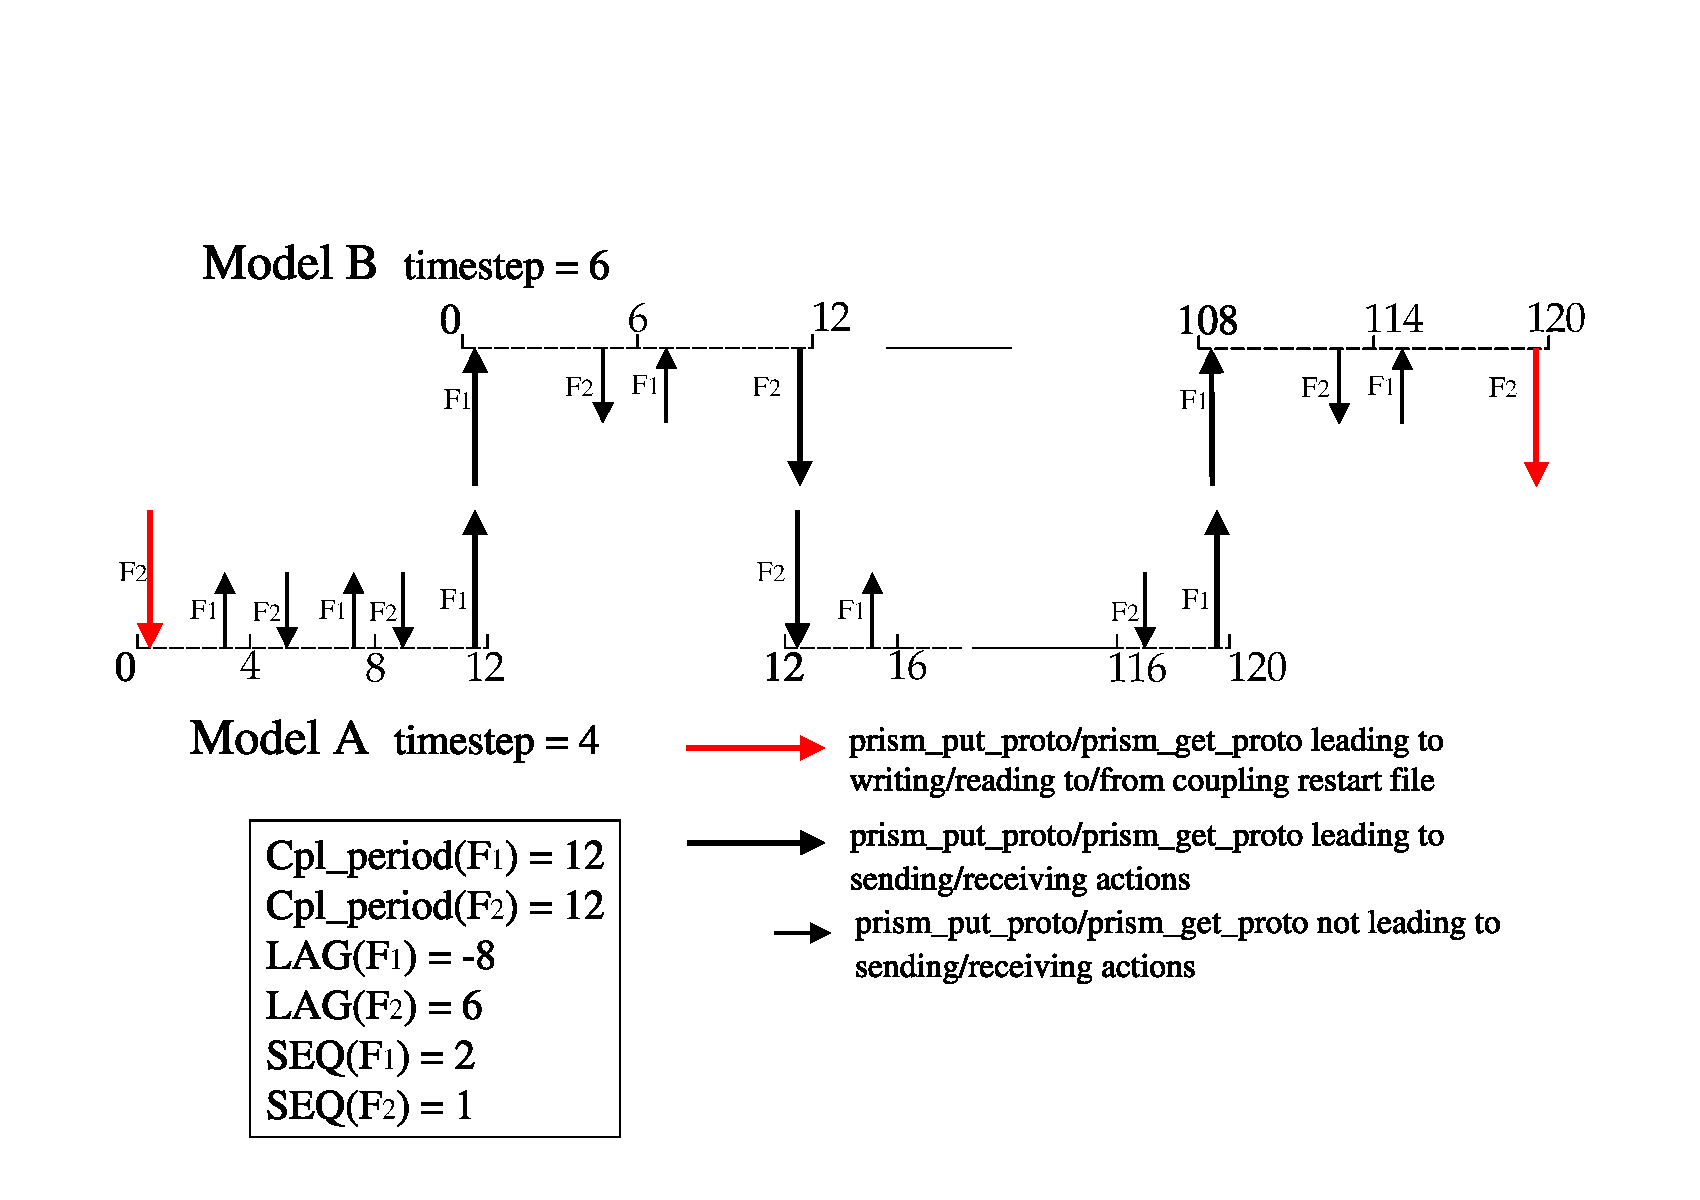
\includegraphics[scale=.6]{figures/fig_mix_seqlag}
%\caption{Mix of LAG and SEQ concepts}
%\label{fig:mix_seqlag}
%\end{figure}
%
%As the LAG for $F_2$ is positive (6), a reading of $F_2$ in its
%coupling restart file is automatically performed by OASIS3 to fulfill the initial
%{\tt prism\_get\_proto}. As the LAG for $F_1$ is negative (-8), no
%reading from file is performed initially and model B waits; at time 8,
%a sending action is effectively performed below model A $F_1$ {\tt
%prism\_put\_proto} (as 8 + LAG (-8) = 0 which is the first coupling
%timestep) and matches the initial model B $F_1$ {\tt
%prism\_get\_proto}. Below the last model A $F_1$ {\tt
%prism\_put\_proto} of the run at time 116, a sending action is
%effectively performed, as $116 + LAG(-8) = 108$ is a coupling period
%(as the LAG is negative, the field is not written to its coupling
%restart file). Below the last model B $F_2$ {\tt prism\_put\_proto} of
%the run at time 114, a writing of $F_2$ to its restart file is
%performed, as $114 + LAG(6) = 120$ is a coupling period and as the LAG
%is positive.
%
%If the coupling fields are transformed through OASIS3 executable, it
%is important to indicate a sequence index. In fact, at each OASIS3
%coupling timestep, $F_1$ must be necessarily treated after
%$F_2$. Therefore, $SEQ(F_1) = 2$ and $SEQ(F_2) = 1$.
%
%\subsection{Mixing sequential and parallel
%    runs using {\tt prism\_put\_restart\_proto}}
%
%In the example illustrated on figure \ref{restart_ex}, the models
%run sequentially for the first run only and then run
%simultaneously. For the first run, the LAG and SEQ indices must be
%defined as in section \ref{subsubsec_mix}.  After the first run, the
%situation is similar to the one of section \ref{subsub_lag}, and
%positive LAG must be defined for $F_1$ and $F_2$. As their lag is
%positive, their corresponding first {\tt prism\_get\_proto} will
%automatically lead to reading $F_1$ and $F_2$ from coupling restart
%files.  In this case, model A has to write $F_1$ to its restart file
%explicitly by calling {\tt prism\_put\_restart\_proto} (illustrated
%on the figure by an orange arrow) at the end of the first run; in
%fact, $F_1$ lag being then negative, such writing is not automatically
%done below the last {\tt prism\_put\_proto} of the first run.
%
%
%\begin{figure}
%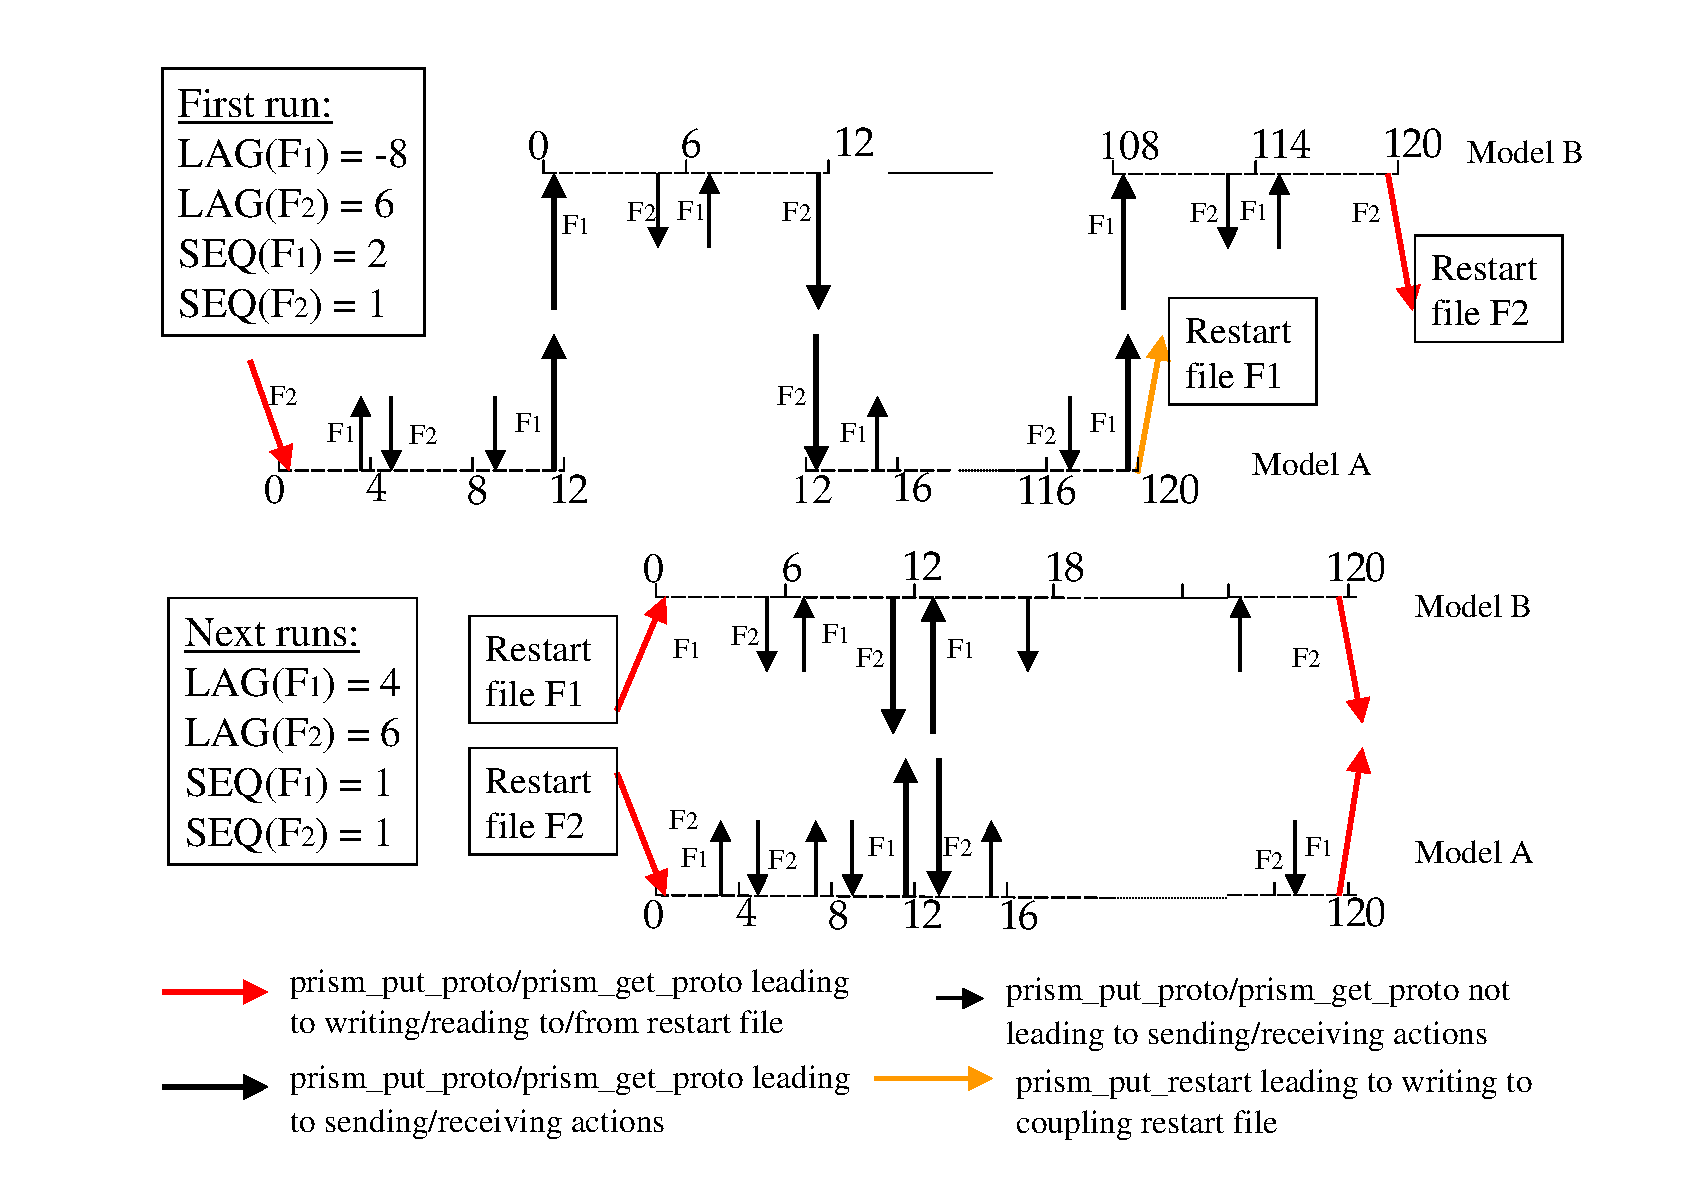
\includegraphics[scale=.6]{figures/restart_example} 
%\caption{An example using prism\_put\_restart\_proto}
%\label{restart_ex}
%\end{figure} 

%section{PRISM System Model Interface for the CLIM/MPI2-MPI1
%communication technique (PSMILe V.0)}
%section{Model\_interfacing} 
